\documentclass[10pt,border=4pt]{standalone}
\usepackage{mathptmx}
\usepackage{amsmath,amssymb,bm}
\usepackage{tikz}
\usetikzlibrary{patterns,decorations.pathmorphing,decorations.pathreplacing,arrows.meta,fit,backgrounds,calc,positioning,shapes.geometric}
\definecolor{acc}{HTML}{0B5394}
\definecolor{accl}{HTML}{EAF0F7}
\definecolor{grp}{HTML}{F5F5F5}
\definecolor{org}{HTML}{C55A11}
\definecolor{orgl}{HTML}{FBEFE6}
\tikzset{
 dat/.style={draw=black,line width=0.6pt,fill=white,align=center,font=\small,inner sep=3pt,minimum height=0.85cm},
 lay/.style={draw=acc,line width=0.8pt,fill=accl,rounded corners=2pt,align=center,font=\small,inner sep=3pt,minimum height=0.85cm},
 cnd/.style={draw=org,line width=0.8pt,fill=orgl,rounded corners=2pt,align=center,font=\small,inner sep=3pt,minimum height=0.75cm},
 op/.style={circle,draw=black,line width=0.6pt,fill=white,inner sep=0.5pt,font=\small,minimum size=5mm},
 grpb/.style={draw=black!45,dashed,line width=0.6pt,rounded corners=3pt,inner sep=6pt},
 arr/.style={-{Latex[length=2.2mm,width=1.7mm]},line width=0.7pt},
 carr/.style={-{Latex[length=2.2mm,width=1.7mm]},line width=0.7pt,draw=org},
 shp/.style={font=\scriptsize,text=black!70,inner sep=1pt},
 lab/.style={font=\footnotesize,inner sep=1pt},
 ttl/.style={font=\small\bfseries,inner sep=0pt,anchor=west}
}
\newcommand{\xh}{\mathbf{x}_h}\newcommand{\xf}{\mathbf{x}_f}

\tikzset{vf/.style={draw=org,line width=0.8pt,fill=orgl},vh/.style={draw=black!70,line width=0.8pt,fill=black!25},
 flow/.style={-{Latex[length=2.0mm,width=1.6mm]},line width=0.9pt,draw=acc}}
\begin{document}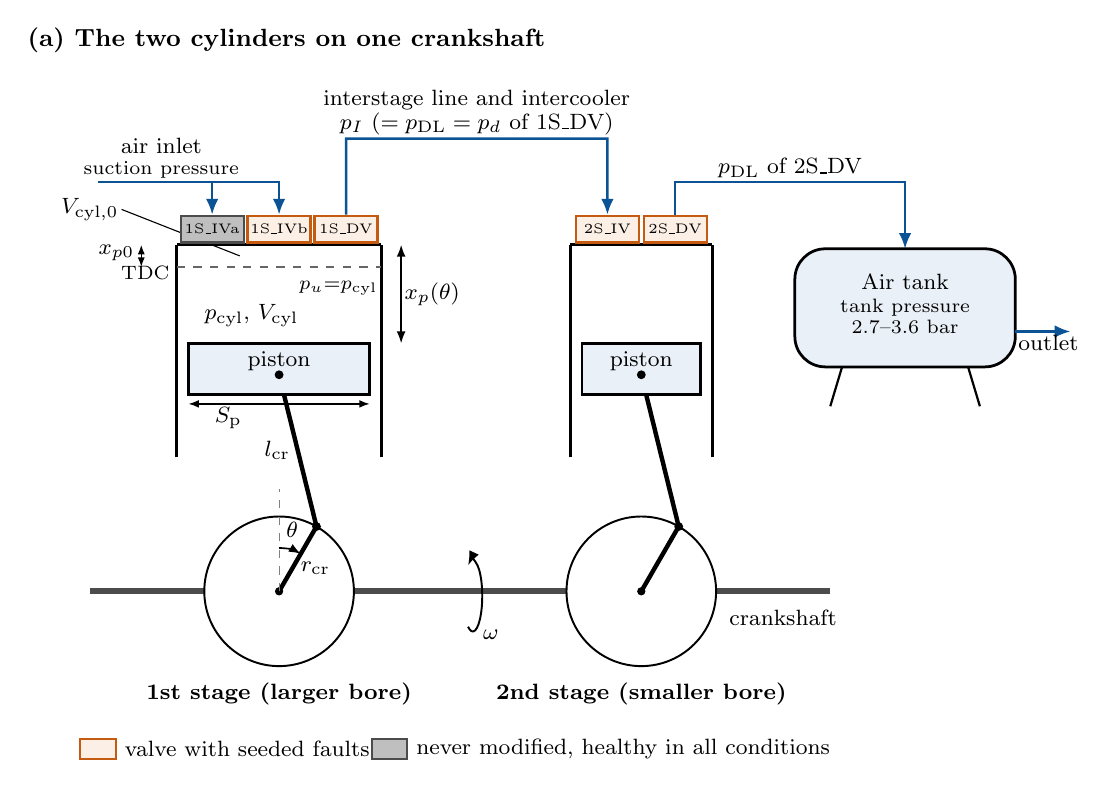
\begin{tikzpicture}[x=1cm,y=1cm]
\node[ttl] at (-0.6,7.0) {(a) The two cylinders on one crankshaft};
% ---------- shaft
\draw[line width=2.2pt,black!70] (0.2,0)--(9.6,0); \node[lab,anchor=north] at (9.0,-0.2) {crankshaft};
% ---------- stage 1 (large bore), centre x=2.6
\begin{scope}[shift={(2.6,0)}]
\draw[line width=0.7pt,fill=white] (0,0) circle (0.95); \fill (0,0) circle (1.5pt);
\coordinate (C) at (60:0.95); \draw[line width=1.6pt] (0,0)--node[lab,below right=-1pt]{$r_\text{cr}$}(C);
\coordinate (P) at (0,2.75); \draw[line width=1.6pt] (C)--node[lab,left=1pt]{$l_\text{cr}$}(P); \fill (C) circle (1.6pt);
\draw[line width=0.9pt,fill=accl] (-1.15,2.5) rectangle (1.15,3.15); \fill (P) circle (1.6pt); \node[lab] at (0,2.92) {piston};
\draw[line width=1pt] (-1.3,1.7)--(-1.3,4.4) (1.3,1.7)--(1.3,4.4);
\draw[line width=1pt] (-1.3,4.4)--(1.3,4.4);
\node[lab] at (-0.35,3.5) {$p_\text{cyl}$, $V_\text{cyl}$};
\draw[{Latex[length=1.5mm]}-{Latex[length=1.5mm]},line width=0.5pt] (1.55,4.4)--node[lab,right]{$x_p(\theta)$}(1.55,3.15);
\draw[dashed,black!50] (0,0)--++(0,1.3); \draw[-{Latex[length=1.5mm]},line width=0.6pt] (0,0.55) arc (90:60:0.55); \node[lab] at (78:0.8) {$\theta$};
% clearance at top dead centre
\draw[dashed,line width=0.5pt,black!60] (-1.3,4.12)--(1.3,4.12); \node[lab,anchor=east,font=\scriptsize] at (-1.35,4.05) {TDC};
\draw[{Latex[length=1.2mm]}-{Latex[length=1.2mm]},line width=0.5pt] (-1.75,4.4)--(-1.75,4.12); \node[lab,anchor=east] at (-1.8,4.3) {$x_{p0}$};
\draw[line width=0.4pt] (-0.5,4.26)--(-2.0,4.85) node[lab,anchor=east]{$V_{\text{cyl},0}$};
\draw[{Latex[length=1.3mm]}-{Latex[length=1.3mm]},line width=0.5pt] (-1.15,2.38)--node[lab,below,pos=0.22]{$S_\text{p}$}(1.15,2.38);
% forces on the 1S_DV plate
\node[lab,font=\scriptsize] at (0.75,3.85) {$p_u{=}p_\text{cyl}$};
% valves on head
\node[vh,minimum width=0.8cm,minimum height=0.34cm,font=\tiny,inner sep=0pt] (va) at (-0.85,4.6) {1S\_IVa}; \node[vf,minimum width=0.8cm,minimum height=0.34cm,font=\tiny,inner sep=0pt] (vb) at (0,4.6) {1S\_IVb}; \node[vf,minimum width=0.8cm,minimum height=0.34cm,font=\tiny,inner sep=0pt] (vd1) at (0.85,4.6) {1S\_DV};
\node[lab,font=\footnotesize\bfseries] at (0,-1.3) {1st stage (larger bore)};
\draw[flow] (-2.3,5.2)--node[lab,above,pos=0.35,align=center]{air inlet\\[-2pt]\scriptsize suction pressure}(0,5.2)--(vb.north); \draw[flow] (-0.85,5.2)--(va.north);
\end{scope}
% ---------- stage 2 (small bore), centre x=7.2
\begin{scope}[shift={(7.2,0)}]
\draw[line width=0.7pt,fill=white] (0,0) circle (0.95); \fill (0,0) circle (1.5pt);
\coordinate (C) at (60:0.95); \draw[line width=1.6pt] (0,0)--(C);
\coordinate (P) at (0,2.75); \draw[line width=1.6pt] (C)--(P); \fill (C) circle (1.6pt);
\draw[line width=0.9pt,fill=accl] (-0.75,2.5) rectangle (0.75,3.15); \fill (P) circle (1.6pt); \node[lab] at (0,2.92) {piston};
\draw[line width=1pt] (-0.9,1.7)--(-0.9,4.4) (0.9,1.7)--(0.9,4.4);
\draw[line width=1pt] (-0.9,4.4)--(0.9,4.4);
\node[vf,minimum width=0.8cm,minimum height=0.34cm,font=\tiny,inner sep=0pt] (iv2) at (-0.43,4.6) {2S\_IV}; \node[vf,minimum width=0.8cm,minimum height=0.34cm,font=\tiny,inner sep=0pt] (dv2) at (0.43,4.6) {2S\_DV};
\node[lab,font=\footnotesize\bfseries] at (0,-1.3) {2nd stage (smaller bore)};
\draw[flow] (dv2.north)--(0.43,5.2)--node[lab,above,align=center]{$p_\text{DL}$ of 2S\_DV}(3.35,5.2)--(3.35,4.35);
\end{scope}
\draw[-{Latex[length=1.8mm]},line width=0.7pt] (5.0,-0.45) arc (-120:120:0.12 and 0.45); \node[lab,anchor=west] at (5.15,-0.55) {$\omega$};
% ---------- tank
\begin{scope}[shift={(10.55,3.6)}]
\draw[line width=1pt,fill=accl,rounded corners=11pt] (-1.4,-0.75) rectangle (1.4,0.75);
\node[lab,align=center] at (0,0.05) {Air tank\\[-1pt]\scriptsize tank pressure\\[-2pt]\scriptsize 2.7--3.6 bar};
\draw[line width=0.8pt] (-0.8,-0.75)--(-0.95,-1.25) (0.8,-0.75)--(0.95,-1.25);
\draw[flow] (1.4,-0.3)--node[lab,below,pos=0.6]{outlet}(2.1,-0.3);
\end{scope}
% ---------- interstage line
\draw[flow] (vd1.north)--(3.45,5.75)--node[lab,above,align=center]{interstage line and intercooler\\[-1pt]$p_I$ ($=p_\text{DL}=p_d$ of 1S\_DV)}(6.77,5.75)--(iv2.north);
% legend
\node[vf,minimum width=0.45cm,minimum height=0.25cm] at (0.3,-2.0) {}; \node[lab,anchor=west] at (0.6,-2.0) {valve with seeded faults};
\node[vh,minimum width=0.45cm,minimum height=0.25cm] at (4.0,-2.0) {}; \node[lab,anchor=west] at (4.3,-2.0) {never modified, healthy in all conditions};
\end{tikzpicture}\end{document}
